\documentclass[10pt,letterpaper,unboxed,cm]{hmcpset}
\usepackage[margin=1in]{geometry}
\usepackage{graphicx, xcolor}
\usepackage{varwidth,multicol}
\pagestyle{empty}

\newcommand{\cmd}[1]{\texttt{\color{blue}{#1}}}

\newcommand{\st}{~\mid~}
\newcommand{\derives}{\implies}

\name{}
\class{CSE 105} 
\assignment{Individual Homework 5}
\duedate{Due: Tuesday May 15, 2018 at 11:00PM (on Gradescope)}

\begin{document}

\begin{center}
\begin{minipage}[t]{5.7in}
\rule{\linewidth}{2pt}
{\sc Instructions}\newline
This {\bf Individual HW5} must be completed without any collaboration
with other students in this class.  The only allowed sources of help for this homework 
are the class textbook, notes, and podcast, and the instructional team.\\


Your homework {\bf must be typed}.  We recommend that you submit early drafts to Gradescope so that in 
case of any technical difficulties, at least some of your work is present.  You may update
your submission as many times as you'd like up to the deadline.\\


{\sc Reading} Sipser Sections 3.1, 3.2, 3.3
\newline

{\sc Key Concepts} Formal definitions of Turing machines, computations of Turing machines,
halting computations, implementation-level descriptions of Turing machines, recognizable languages, decidable languages.\newline

\rule{\linewidth}{2pt}
\end{minipage} \hfill

\end{center}

\problemlist{}



\begin{problem}[1.]({\bf 10 points}) The alphabet for this question is $\{0,1,2\}$. The state diagrams of the Turing machines for this question are on the last page
of the assignment. For each question below, list {\bf all} the machines from the list $M_1, M_2, 
M_3, M_4, M_5$ for which the answer is ``yes", or write {\bf None} otherwise.
\begin{itemize}
\item[a.] Which of the machines accept the string $0$?
\item[b.] Which of the machines accept the string $\varepsilon$?
\item[c.] For which of these machines is it true that the contents of the tape are never changed during a computation?
\item[d.] Which of the machines recognize the set $\emptyset$?
\item[e.] Which of the machines decide the set $\emptyset$?
\item[f.] For which of these machines is it true that on at least one input, the computation of the machine halts
and that on at least one input, the computation of the machine does not halt?
\end{itemize}



{\it No justifications required for credit for this question; but, as always, they're a good idea for your own benefit.}
\end{problem}

\begin{problem}[2.]  ({\bf 10 points}). 
The alphabet for this question is $\{0,1,2\}$. The state diagrams of the Turing machines for this question are on the last page
of the assignment. 
\begin{itemize}
\item[a.] The implementation-level description below is {\bf not} a description of $M_2$.
\begin{quote}
``On input $w$:
\begin{itemize}
\item[1.] If $w$ is the empty string, accept.  
\item[2.] Otherwise, sweep through the tape from left to right, erasing all input characters, until you reach the end of $w$, and accept."
\end{itemize}
\end{quote}
(i) Change item 2 above to get an implementation-level description that does describe $M_2$. 

(ii) When $w$ is of length $k$ ($k >0$), how many steps are there in the computation of $M_2$ on $w$? \\


\item[b.] In this part of the problem, you will write the formal definition for a new machine that is related to $M_4.$
The new Turing machine is described by the  implementation-level description:
\begin{quote}
``On input $w$:
\begin{itemize}
\item[1.] If $w$ is the empty string, reject.  
\item[2.] Otherwise, scan through the tape from left to right until you reach the end of $w$, and accept."
\end{itemize}
\end{quote}

(i) Fill in the blanks below to define the machine described by this implementation-level description:
\[
M = (\{q_0, q_1, q_{acc}, q_{rej}\}, \{0,1,2\}, \{0,1,2, \square\}, \delta, q_0, q_{acc}, q_{rej} )
\]
 where
\begin{align*}
\delta( (q_0, \square) ) &= \underline{\phantom{FILL IN BLANK HERE}} \\
\delta ( (q_0 ,x) ) &= \underline{\phantom{FILL IN BLANK HERE}} \qquad \text{if } x  \in \Sigma \\
\delta( (q_1, \square) ) &= \underline{\phantom{FILL IN BLANK HERE}} \\
\delta ( (q_1 ,x) ) &= \underline{\phantom{FILL IN BLANK HERE}} \qquad \text{if } x  \in \Sigma \\
\delta( (q_{acc}, x) ) &= (q_{acc}, \square, L) \qquad \text{if } x \in \Gamma\\
\delta( (q_{rej}, x) ) &= (q_{acc}, \square, L) \qquad \text{if } x \in \Gamma\\
\end{align*}


{\it Hint}: The transition function of the Turing machine $M$ has domain 
\[
\{q_0, q_1, q_{acc}, q_{rej}\} \times \{0,1,2,\square\}
\]
and codomain 
\[
\{q_0, q_1, q_{acc}, q_{rej}\} \times \{0,1,2,\square\} \times \{L, R \}
\]
Make sure the outputs you specify when you fill in the blank are {\bf ordered triples} of the right type.


(ii) What is $L(M)$?

(iii) Is $M$ a decider?


\end{itemize}

{\it No justifications required for credit for this question; but, as always, they're a good idea for your own benefit.}


\end{problem}

\begin{problem}[3.] ({\bf 10 points}) 
Suppose $M_1$ and $M_2$ are Turing machines. Consider the Turing machines given by the
high-level descriptions:
\begin{quote}
``$M$ = On input $w$,
\begin{itemize}
\item[1.] Run $M_1$ on input $w$.  If $M_1$ accepts $w$, accept.  If $M_1$ rejects $w$, go to 2.
\item[2.] Run $M_2$ on input $w$. If $M_2$ accepts $w$, accept.  If $M_2$ rejects $w$, reject."
\end{itemize}
\end{quote}
\begin{quote}
``$\tilde{M}$ = On input $w$,
\begin{itemize}
\item[1.] Run $M_1$ on input $w$.  If $M_1$ rejects $w$, reject.  If $M_1$ accepts $w$, go to 2.
\item[2.] Run $M_2$ on input $w$. If $M_2$ rejects $w$, reject.  If $M_2$ accepts $w$, accept."
\end{itemize}
\end{quote}


For each of the following claims, answer {\bf Always true} if the statement is true for all possible $M_1$
and $M_2$; answer {\bf Always false}  if the statement is false for all possible $M_1$
and $M_2$; and answer {\bf Neither} otherwise.
\begin{itemize}
\item[a.] If $w \in L(M_1)$ then $w \in L(M)$.
\item[b.] If $w \in L(M_2)$ then $w \in L(M)$.
\item[c.] If $w \notin L(M_1)$ then $w \notin L(M)$.
\item[d.] If $w \notin L(M_2)$ then $w \notin L(M)$.
\item[e.] If $w \in L(M)$ then either $w \in L(M_1)$ or $w \in L(M_2)$ or both.
\item[f.] If $w \in L(M_1)$ then $w \in L(\tilde{M})$.
\item[g.] If $w \in L(M_2)$ then $w \in L(\tilde{M})$.
\item[h.] If $w \notin L(M_1)$ then $w \notin L(\tilde{M})$.
\item[i.] If $w \notin L(M_2)$ then $w \notin L(\tilde{M})$.
\item[j.] If $w \in L(M_1)$  and $w \in L(M_2)$ then $w \in L(\tilde{M})$.
\end{itemize}


{\it No justifications required for credit for this question; but, as always, they're a good idea for your own benefit.}


\end{problem}

\newpage
\begin{center}
{\bf State diagrams of Turing machines for Problems 1 and 2}.  Recall that the alphabet is $\Sigma = \{0,1,2\}$.\\

\begin{tabular}{| c  c |}
\hline
$M_1$ & 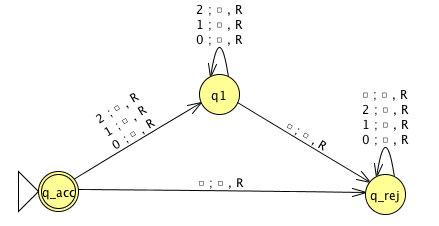
\includegraphics[width=3.5in]{TMex1_HW5.png} \\
\hline
\hline
$M_2$ & 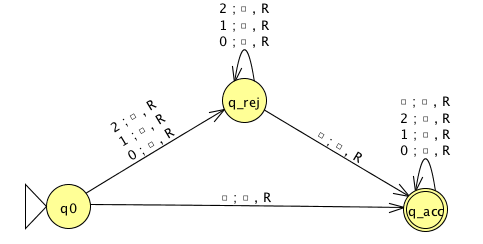
\includegraphics[width=3.5in]{TMex2_HW5.png} \\
\hline
\hline
$M_3$ & 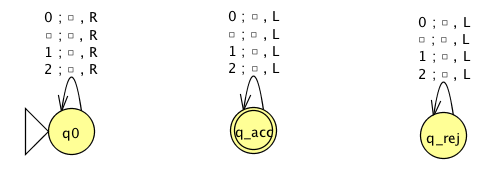
\includegraphics[width=3.5in]{TMex3_HW5.png} \\
\hline
\hline
$M_4$ & 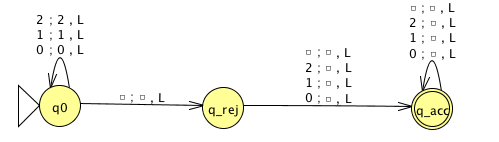
\includegraphics[width=3.5in]{TMex4_HW5.png} \\
\hline
\hline
$M_5$ & 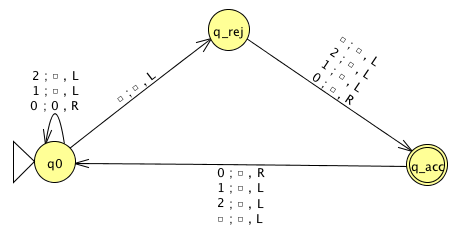
\includegraphics[width=3.5in]{TMex5_HW5.png} \\
\hline
\end{tabular}

\end{center}

\end{document}
